%%%%%%%%%%%%%%%%%%%%%%%%%%%%%%%%%%%%%%%%%%%%%%%
%%% Template for lab reports used at BIT modified from STIMA
%%%%%%%%%%%%%%%%%%%%%%%%%%%%%%%%%%%%%%%%%%%%%%%

%%%%%%%%%%%%%%%%%%%%%%%%%%%%%% Sets the document class for the document
% Openany is added to remove the book style of starting every new chapter on an odd page (not needed for reports)
\documentclass[11pt,english, openany]{book}
%%%%%%%%%%%%%%%%%%%%%%%%%%%%%% Loading packages that alter the style
\usepackage[]{graphicx}
\usepackage[]{color}
\usepackage{alltt}
%\usepackage[T1]{fontenc}
\usepackage[utf8]{inputenc}
\setcounter{secnumdepth}{3}
\setcounter{tocdepth}{3}
\setlength{\parskip}{\smallskipamount}
\setlength{\parindent}{12pt}

% Set page margins
\usepackage[top=60pt,bottom=60pt,left=68pt,right=66pt]{geometry}
\usepackage{subcaption}
% Package used for placeholder text
\usepackage{lipsum}
\usepackage{booktabs}
\usepackage{multirow}
% Prevents LaTeX from filling out a page to the bottom
\raggedbottom

% Adding both languages
\usepackage[english]{babel}

% All page numbers positioned at the bottom of the page
\usepackage{fancyhdr}
\fancyhf{} % clear all header and footers
\fancyfoot[C]{\thepage}
\renewcommand{\headrulewidth}{0pt} % remove the header rule
\pagestyle{fancy}

% Changes the style of chapter headings
\usepackage{titlesec}
\titleformat{\chapter}
   {\normalfont\LARGE\bfseries}{\thechapter.}{1em}{}
% Change distance between chapter header and text
\titlespacing{\chapter}{0pt}{40pt}{2\baselineskip}

% Adds table captions above the table per default
\usepackage{float}
\floatstyle{plaintop}
\restylefloat{table}

% Adds space between caption and table
\usepackage[tableposition=top]{caption}

% add cc license
\usepackage[
type={CC},
modifier={by-nc-sa},
version={4.0},
]{doclicense}

% Adds hyperlinks to references and ToC
\usepackage{hyperref}
% Uncomment the line below this block to set all hyperlink color to black
\hypersetup{
	colorlinks,
	linkcolor={blue},
	citecolor={green!90!black},
	urlcolor={red!70!black}
}
%\hypersetup{hidelinks,linkcolor = black} % Changes the link color to black and hides the hideous red border that usually is created

% Set specific color for hyperref
\usepackage{xcolor}


% tcolorbox; Notice! add "-shell-escape" to the compile command
\usepackage{tcolorbox}

% If multiple images are to be added, a folder (path) with all the images can be added here 
\graphicspath{ {Figures/} }

% Separates the first part of the report/thesis in Roman numerals
\frontmatter


%%%%%%%%%%%%%%%%%%%%%%%%%%%%%% Starts the document
\begin{document}

%%% Selects the language to be used for the first couple of pages
\selectlanguage{english}

%%%%% Adds the title page
\begin{titlepage}
	\clearpage\thispagestyle{empty}
	\centering
	\vspace{1cm}

	% Titles
	% Information about the University
	{\normalsize \textbf{\textit{Course name}} \\ 
		Beijing Institute of Technology \par}
		\vspace{5.5cm}
	{\Huge \textbf{PROJECT NAME}} \\
	\vspace{0.6cm}
	{\large \textbf{PROJECT TITLE} \par}
	\vspace{4.3cm}
	{\normalsize James Bond \\ % \\ specifies a new line
	             0000000 \\
	             1120202222\par}
	\vspace{2.6cm}
    
    \centering 
\includegraphics[scale=0.6]{bit_logo.pdf}\\
    \centering 
\includegraphics[scale=0.4]{logo_slogan.pdf}
    \vspace{0.5cm}

		
	% Set the date
	{\normalsize May-2020 \par}
	
	\pagebreak

\end{titlepage}

% Adds a table of contents keep the link black
{\hypersetup{linkcolor=black}
	% or \hypersetup{linkcolor=black}, if the colorlinks=true option of hyperref is used
	\tableofcontents{}
}

%%%%%%%%%%%%%%%%%%%%%%%%%%%%%%%%%%%%%%%%%%%%%%%%%%%%%%%%%%%%%%%%%%%%%%%%%%%%%%%%%%%%%%%%%%%%
%%%%%%%%%%%%%%%%%%%%%%%%%%%%%%%%%%%%%%%%%%%%%%%%%%%%%%%%%%%%%%%%%%%%%%%%%%%%%%%%%%%%%%%%%%%%
%%%%% Text body starts here!
\mainmatter

% Comment the following two lines to remove abstract 
\chapter*{\makebox[\linewidth]{Abstract}}
\addcontentsline{toc}{chapter}{Abstract}
\lipsum[5]

\vspace{0.5cm}
\noindent\textbf{Keywords}: 
LaTex, BIT

\chapter{Problem Statement}\label{chapt:problem}

\lipsum[1-2]

\section{Requirements} 

\begin{figure}[h]
	\centering
	\subfloat[My simulationrun on Windows]{{\includegraphics[width=6.5cm]{single_sine_perturb} }}%
	\qquad
	\subfloat[My simulation run on Linux]{{\includegraphics[width=6.5cm]{single_sine_perturb} }}%
	\caption{Two figure example 1}%
	\label{fig:Two figure}%
\end{figure}


\chapter{Introduction}\label{chapt:intro}



\lipsum[1]

\vspace{0.6cm}
\begin{tcolorbox}[title=\textbf{tcolorbox example}]
	\lipsum[2]
\end{tcolorbox}

\chapter{Part two}
Citation is used like\cite{ex}.

\begin{figure}[H]
	\centering
	\begin{subfigure}{0.49\linewidth} \centering
		\includegraphics[scale=0.25]{Figures/single_sine_perturb}
		\caption{S.C.L with sinusoidal disturbance}\label{fig:figA}
	\end{subfigure}
	\begin{subfigure}{0.49\linewidth} \centering
		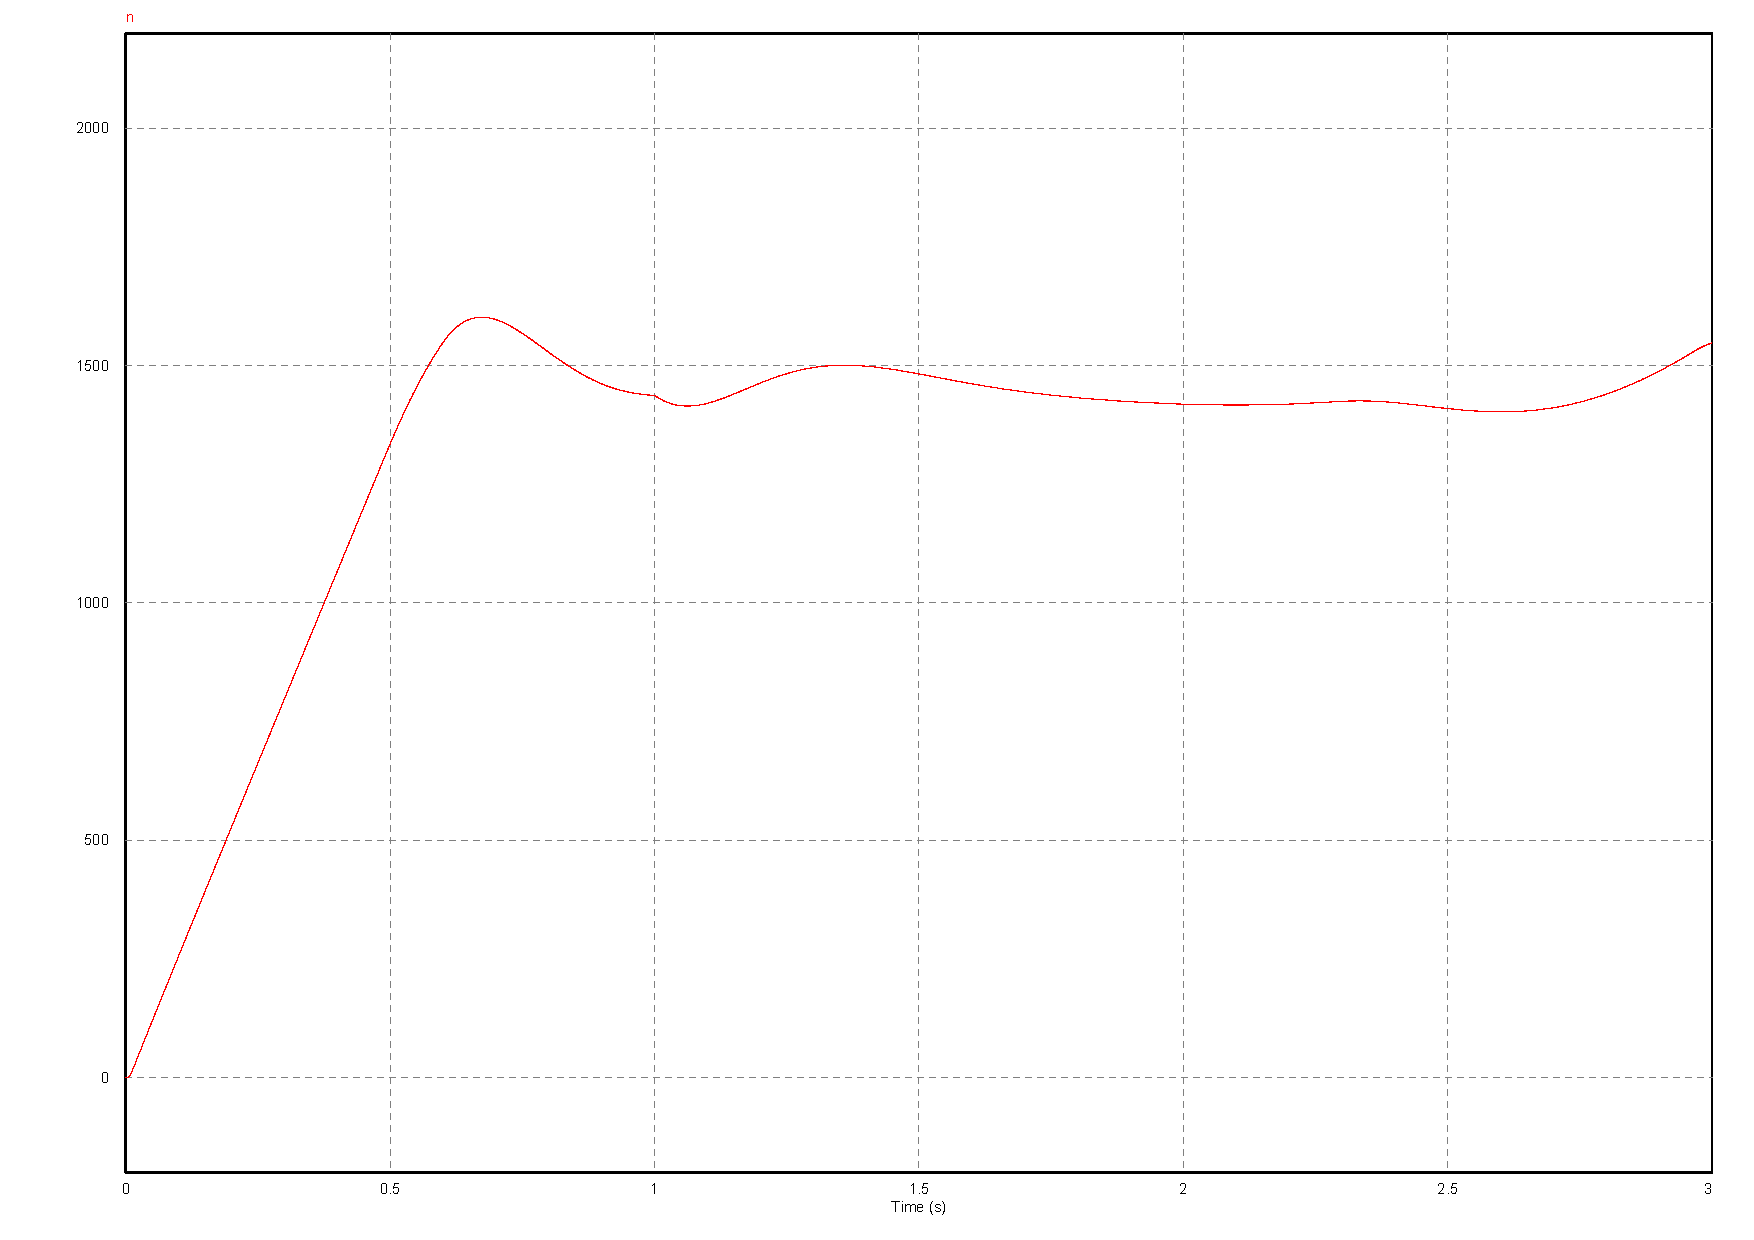
\includegraphics[scale=0.25]{Figures/dual_sine_perturb}
		\caption{D.C.L with sinusoidal disturbance}\label{fig:figB}
	\end{subfigure}
	\caption{Two figure example 2} \label{fig:twodisturb}
\end{figure}
\chapter{Conclusions}

\lipsum[2]


\begin{table}[b]
	\centering
	\small
	\begin{tabular}{lccc}
		\toprule
		\multirow{2}{*}{Speed Regulation System} & \multicolumn{3}{c}{Performances} \\ \cmidrule(lr){2-4}
		& Start up &  Under disturbance &  Cost \\
		\midrule
		Single Closed Loop speed regulation system  & faster & more robust & more complicated and pricey \\
		Dual Closed Loop speed regulation system & slower & less robust & simple and cheap \\
		\bottomrule
	\end{tabular}
	\caption{The Comparison Between Two Systems}
	\label{tab-label-1}
\end{table}

\lipsum[3-5]

\pagebreak

% Adding a bibliography if citations are used in the report
% Uncomment the following line to customize the Bibliography title
%\renewcommand{\bibname}{References}
\bibliographystyle{plain}
\bibliography{ref}

% Uncomment the following two lines to remvoe the cc license
\vspace*{\fill}
{\hypersetup{urlcolor=black}{\footnotesize \doclicenseThis}}
% Adds reference to the Bibliography in the ToC
\addcontentsline{toc}{chapter}{\bibname}

\pagebreak

%\chapter*{Appendix A: Resources}
%[\textit{Report the config files of the software used (i.e. SU2  and the mesher). Also attach to this report an archive with the mesh files, solutions and the reference solution data (e.g. data points of a Cp plot ...)}]
%\section*{Mesh configuration files}
%\section*{SU2 configuration files}
%% \section{Reference solution data}


\end{document}
